\section{Моделирование электронно-стимулированных разрывов полимерных молекул} \label{sec:G_value}
Количественной характеристикой процесса электронно-стимулированной деградации полимерного резиста является радиационно-химический выход разрывов $\Gs$, определяемый как число разрывов полимерных молекул, происходящих при выделении в слое резиста энергии 100 эВ.
Экспериментально $\Gs$ определяется на основе значений среднечисловой молекулярной массы резиста до и после экспонирования ($\Mn$ и $M_\mathrm{f}$, соответственно), определяемых методом гель-проникающей хроматографии.
При известных $\Mn$ и $M_\mathrm{f}$ значение $\Gs$ может быть определено на основе выражения~\cite{Greeneich1979_Mf_Mn}
\begin{equation} \label{eq:G_value_Mn_Mf}
	M_\mathrm{f} = \frac{\displaystyle \Mn}{1 + \frac{\displaystyle \Gs E}{\displaystyle 100 \rho N_\mathrm{A}}},
\end{equation}
где $E$ -- энергия, выделившаяся в слое резиста, $\rho$ -- плотность резиста, $N_\mathrm{A}$ -- число Авогадро.

Исходя из результатов различных экспериментов по измерению $\Gs$, его значение для ПММА при экспонировании электронным лучом при комнатной температуре считается равным 1.8~\cite{Charlesby_1964_Gs}. Также было установлено, что при экспонировании гамма-излучением и электронным лучом при различных температурах ($T$) зависимость $\ln \Gs (1/T)$ близка к линейной (рисунок~\ref{fig:Gs_Charlesby}).

Считается, что электронно-стимулированные разрывы молекул ПММА происходят в результате взаимодействия налетающего электрона с валентными электронами атомов углерода, образующими C---C связь в главной цепи молекулы~\cite{Stepanova_2006}.

\begin{figure}[h]
	\begin{center}
		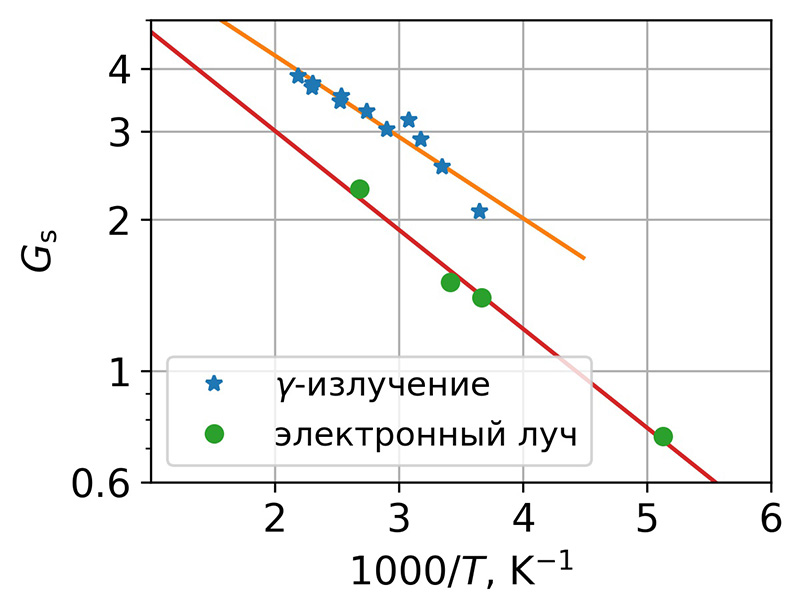
\includegraphics[width=0.55\linewidth]{jpg/Charlesby_G_fit_200}
		\caption{Значения $G_\mathrm{s}$ для ПММА при экспонировании гамма-излучением и электронным лучом, полученные при различных температурах~\cite{Charlesby_1964_Gs}. Сплошная линия отображает аппроксимацию экспериментальных значений $\ln(G_\mathrm{s})$ функцией вида $\alpha\cdot1/T$.}
		\label{fig:Gs_Charlesby}
	\end{center}
\end{figure}
